\documentclass{article}

\usepackage[utf8]{inputenc}
\usepackage[T1]{fontenc}
\usepackage[ngerman]{babel}
\usepackage{amsmath, amsfonts, amsthm, mathtools, amssymb}
\usepackage{stmaryrd}
\usepackage{enumerate}
\usepackage{cases}
\usepackage{fancyhdr}
\usepackage{comment}
%\usepackage{xcolor}
\usepackage{tikz}
\usepackage{pgf}
\usepackage{pgfplots}
\pgfplotsset{compat=1.16}
\usepackage{cases}
\usepackage{listings}
\usepackage{siunitx}
\usepackage[left = 3cm, bottom =3cm]{geometry}
\usepackage[hidelinks]{hyperref}
\usepackage{subcaption}
\usepackage{gauss}
\usepackage{nicematrix}
\usepackage{graphicx}

\usepackage{environ}
\newtheorem{satz}{Satz}[section]
\newtheorem{lemma}[satz]{Lemma}
\newtheorem{korollar}[satz]{Korollar}
\newtheorem{proposition}[satz]{Proposition}
\theoremstyle{definition}
\newtheorem{definition}[satz]{Def.}
\newtheorem{axiom}[satz]{Axiom}
\newtheorem{bsp}[satz]{Bsp.}
\newtheorem*{anmerkung}{Anm}
\newtheorem{bemerkung}[satz]{Bem}
\newtheorem*{notatio}{Notation}
\newcommand{\obda}{O.B.d.A. }
\newcommand{\equals}{\Longleftrightarrow}
\newcommand{\N}{\mathbb{N}}
\newcommand{\Q}{\mathbb{Q}}
\newcommand{\R}{\mathbb{R}}
\newcommand{\Z}{\mathbb{Z}}
\newcommand{\C}{\mathbb{C}}
\newcommand{\K}{\mathbb{K}}
\newcommand{\intd}{\mathrm{d}}
\newcommand{\Pot}{\operatorname{Pot}}
\newcommand{\mychar}{\operatorname{char}}
\newcommand{\myker}{\operatorname{ker}}
\newcommand{\induktion}[3]
{\begin{proof}\ \\
	\noindent\textbf{Induktionsanfang:}\ #1\\
	\noindent\textbf{Induktionsvoraussetzung:}\ #2\\
	\noindent\textbf{Induktionsschluss:}\ #3
\end{proof}}

\newcommand{\rg}{\operatorname{rg}}
\newcommand{\im}{\operatorname{im}}
\newcommand{\End}{\operatorname{End}}
\newcommand{\abb}{\operatorname{Abb}}
\newcommand{\re}{\operatorname{Re}}
\newcommand{\Ima}{\operatorname{Im}}

\let\oldstackrel\stackrel
\renewcommand{\stackrel}[2]{%
    \oldstackrel{\mathclap{#1}}{#2}
}%


\newcommand{\numlayout}[1]
{	
	\pagestyle{fancy}
	\fancyhead[L]{Einführung in die Numerik, Blatt #1}
	\fancyhead[R]{David Wesner, Josua Kugler}
	\fancypagestyle{firstpage}{%
		\fancyhf{}
		\lhead{Professor: Peter Bastian\\
			Tutor: Ernestine Großmann}
		\rhead{Einführung in die Numerik, Übungsblatt #1\\ David, Josua}
		\cfoot{\thepage}
	}
\thispagestyle{firstpage}
}

\newcommand{\analayout}[1]
{	
	\pagestyle{fancy}
	\fancyhead[L]{Analysis 2, Blatt #1}
	\fancyhead[R]{David Wesner, Josua Kugler}
	\fancypagestyle{firstpage}{%
		\fancyhf{}
		\lhead{Professor: Ekaterina Kostina\\
			Tutor: Julian Matthes}
		\rhead{Analysis 1, Übungsblatt #1\\ David Wesner, Josua Kugler}
		\cfoot{\thepage}
	}
	\thispagestyle{firstpage}
}
\newcommand{\lalayout}[1]
{	
	\pagestyle{fancy}
	\fancyhead[L]{Lineare Algebra 2, Blatt #1}
	\fancyhead[R]{David Wesner, Josua Kugler}
	\fancypagestyle{firstpage}{%
		\fancyhf{}
		\lhead{Professor: Denis Vogel\\
			Tutor: Marina Savarino}
		\rhead{Lineare Algebra 2, Übungsblatt #1\\ David Wesner, Josua Kugler}
		\cfoot{\thepage}
	}
	\thispagestyle{firstpage}
}

\lstset{
    frame=tb, % draw a frame at the top and bottom of the code block
    tabsize=4, % tab space width
    showstringspaces=false, % don't mark spaces in strings
    numbers=left, % display line numbers on the left
    commentstyle=\color{green}, % comment color
    keywordstyle=\color{blue}, % keyword color
    stringstyle=\color{red} % string color
}
\setlength{\headheight}{25pt}

\makeatletter \renewcommand\d{\ensuremath{%
		\;\mathrm{d}}}
\makeatother

\ExplSyntaxOn

% S-tackrelcompatible ALIGN environment
% some might also call it the S-uper ALIGN environment
% uses regular expressions to calculate the widest stackrel
% to put additional padding on both sides of relation symbols
\NewEnviron{salign}
{
    \begin{align}
        \lec_insert_padding:V \BODY
    \end{align}
}
% starred version that does no equation numbering
\NewEnviron{salign*}
{
    \begin{align*}
        \lec_insert_padding:V \BODY
    \end{align*}
}

% some helper variables
\tl_new:N \l__lec_text_tl
\seq_new:N \l_lec_stackrels_seq
\int_new:N \l_stackrel_count_int
\int_new:N \l_idx_int
\box_new:N \l_tmp_box
\dim_new:N \l_tmp_dim_a
\dim_new:N \l_tmp_dim_b
\dim_new:N \l_tmp_dim_needed

% function to insert padding according to widest stackrel
\cs_new_protected:Nn \lec_insert_padding:n
 {
  \tl_set:Nn \l__lec_text_tl { #1 }
  % get all stackrels in this align environment
  \regex_extract_all:nnN { \c{stackrel}{(.*?)}{(.*?)} } { #1 } \l_lec_stackrels_seq
  % get number of stackrels
  \int_set:Nn \l_stackrel_count_int { \seq_count:N \l_lec_stackrels_seq }
  \int_set:Nn \l_idx_int { 1 }
  \dim_set:Nn \l_tmp_dim_needed { 0pt }
  % iterate over stackrels
  \int_while_do:nn { \l_idx_int <= \l_stackrel_count_int }
  {
      % calculate width of text
      \hbox_set:Nn \l_tmp_box {$\seq_item:Nn \l_lec_stackrels_seq { \l_idx_int + 1 }$}
      \dim_set:Nn \l_tmp_dim_a {\box_wd:N \l_tmp_box}
      % calculate width of relation symbol
      \hbox_set:Nn \l_tmp_box {$\seq_item:Nn \l_lec_stackrels_seq { \l_idx_int + 2 }$}
      \dim_set:Nn \l_tmp_dim_b {\box_wd:N \l_tmp_box}
      % check if 0.5*(a-b) > minimum padding, if yes updated minimum padding
      \dim_compare:nNnTF
        { 1pt * \dim_ratio:nn { \l_tmp_dim_a - \l_tmp_dim_b } { 2pt } } > { \l_tmp_dim_needed }
        { \dim_set:Nn \l_tmp_dim_needed { 1pt * \dim_ratio:nn { \l_tmp_dim_a - \l_tmp_dim_b } { 2pt } } }
        { }
      \quad
      % increment list index by three, as every stackrel produces three list entries
      \int_incr:N \l_idx_int
      \int_incr:N \l_idx_int
      \int_incr:N \l_idx_int
  }
  % replace all relations with align characters (&) and add the needed padding
  \regex_replace_all:nnN
      { (\c{approx}&|&\c{approx}|\c{equiv}&|&\c{equiv}|=&|&=|\c{le}&|&\c{le}|\c{ge}&|&\c{ge}|&\c{stackrel}{.*?}{.*?}|\c{stackrel}{.*?}{.*?}&|&\c{neq}|\c{neq}&) }
      { \c{kern} \u{l_tmp_dim_needed} \1 \c{kern} \u{l_tmp_dim_needed} }
      \l__lec_text_tl
  \l__lec_text_tl
 }
\cs_generate_variant:Nn \lec_insert_padding:n { V }
\ExplSyntaxOff


% norm
\newcommand{\norm}[1]{\left\Vert#1\right\Vert}
\newcommand{\maxnorm}[1]{\norm{#1}_\infty}
\renewcommand{\epsilon}{\varepsilon}
\newcommand{\pdv}[2]{\frac{\partial #1}{\partial #2}}
\begin{document}
\numlayout{10}
\section*{Aufgabe 1}
Wir verwenden vollständige Induktion nach der Anzahl der Stützstellen. Der Induktionsanfang ist trivial, sei also die Behauptung für $n-1$ Stützstellen bewiesen. Jede Permutation von $n$ Stützstellen lässt sich als Komposition von Vertauschungen zweier Elemente schreiben. Sei also eine Permutation $\tilde{x_1}, \dots, \tilde{x_n}$ von $x_1,\dots, x_n$ gegeben, wobei $\tilde{x_i} = x_j, \tilde{x_j} = x_i$ und sonst $\tilde{x_k} = x_k$ gelte. Dann gilt
\[
    y[x_i, \dots, x_j] = \frac{y[x_{i+1},\dots,x_j] - y[x_i, \dots, x_{j-1}]}{x_j-x_i} = \frac{y[\tilde{x_{i+1}},\dots,\tilde{x_{j-1}}, \tilde{x_i}] - y[\tilde{x_j}, \tilde{x_{i+1}}, \dots, \tilde{x_{j-1}}]}{\tilde{x_i}-\tilde{x_j}}
\]
Nun nutzen wir die Induktionsvoraussetzung. Da $j-i-1 \le n-1$ gilt, können wir die Einträge der $y$ vertauschen. Daher gilt
\[
    y[x_i, \dots, x_j] = \frac{y[\tilde{x_{i}},\dots,\tilde{x_{j-1}}] - y[\tilde{x_{i+1}}, \dots, \tilde{x_{j}}]}{\tilde{x_i}-\tilde{x_j}} = y[\tilde{x_i}, \tilde{x_j}].
\]
Da sonst keine Elemente vertauscht wurden, erhalten wir schon die Behauptung.
\section*{Aufgabe 2}
Es existiert auf jeden Fall eine geeignete Funktion, deren Ableitung gleich der Ableitung der Spline-Funktion an den Rändern ist. Daher werden Hermite-Randbedingungen erfüllt und wir können Satz 21.6 anwenden. Es gilt daher $\max_{x\in [0,1]} |f(x) - s(x)| \le \frac{1}{N^4}\max_{x\in [0,1]}|16\pi^4\sin(2\pi x)| = \frac{16\pi^4}{N}$. Wählen wir also $N = \lceil 2\pi 10^3\rceil$, so erhalten wir $\max_{x\in [0,1]} |f(x) - s(x)| \leq 10^{-12}$.
\section*{Aufgabe 3}
Es gilt $x_0 = 0, y_0 = 0,\; x_1 = \frac{\pi}{2},y_1 = \frac{1}{2},\; x_2 = \pi,y_2 = 1,\; x_3 = \frac{3\pi}{2},y_3 = \frac{1}{2}$. 
Es gilt
\begin{align*}
    c_0 &= \frac{1}{4}\left(y_0 + y_1 + y_2 + y_3\right) = \frac{1}{2}\\
    c_1 &= \frac{1}{4}\left(y_0 + y_1e^{-i\frac{2\pi}{4}} + y_2 e^{-i\frac{4\pi}{4}} + y_3 e^{-i\frac{6\pi}{4}}\right)\\
    &= \frac{1}{4}\left(-i\frac{1}{2} - 1 + i\frac{1}{2}\right) = -\frac{1}{4}\\
    c_2 &= \frac{1}{4}\left(y_0 + y_1e^{-i\frac{4\pi}{4}} + y_2 e^{-i\frac{8\pi}{4}} + y_3 e^{-i\frac{12\pi}{4}}\right)\\
    &= \frac{1}{4}\left(-\frac{1}{2} + 1 - \frac{1}{2}\right) = 0\\
    c_3 &= \frac{1}{4}\left(y_0 + y_1e^{-i\frac{6\pi}{4}} + y_2 e^{-i\frac{12\pi}{4}} + y_3 e^{-i\frac{18\pi}{4}}\right)\\
    &= \frac{1}{4}\left(i\frac{1}{2} - 1 -i\frac{1}{2}\right) = -\frac{1}{4}
\end{align*} 
\section*{Aufgabe 4}
\begin{enumerate}[(a)]
    \item Es gilt
    \begin{align*}
        f_1'(x) &= 2x(x-6) + x^2 - 2(x-2)\\
        f_1''(x)&= 2(x-6) + 2x + 2x - 2\\
        f_1''(x_0)&= 2(0-6) + 0 - 2 \neq 0
    \end{align*}
    Also verletzt $f_1$ die natürlichen Randbedingungen und liegt daher nicht in $S(X)$.
    Schränken wir $f_2$ auf die beiden Teilintervalle ein, so erhalten wir $g \coloneqq f_2|_{[0,1]} = -\frac{1}{2}x^3$ und $h \coloneqq f_2|_{[1,2]} = (x-1)^3 - \frac{1}{2}x^3$. Nun müssen wir die Bedingungen prüfen. Es gilt $g'(x) = - \frac{3}{2}x^2,\; g''(x) = -3x$ und $h'(x) = 3(x-1)^2 - \frac{3}{2}x^2,\; h''(x) = 6(x-1) - 3x$. Die Stetigkeit ist erfüllt wegen $g(1) = -\frac{1}{2} = h(1)$, die Stetigkeit der ersten Ableitung gilt wegen $g'(1) = - \frac{3}{2} = 3(1-1)^2 - \frac{3}{2} = h'(1)$, die Stetigkeit der zweiten Ableitung folgt aus $g''(1) = -3 = 6(1-1) - 3 = h''(x)$ und die Randbedingungen gelten wegen $g''(0) = 0$ und $h''(2) = 6 - 6 = 0$. Also ist $f_2 \in S(X)$.
    Schließlich gilt
    \begin{align*}
        f_3'(x) &= 3x^2 + 2x\\
        f_3''(x) &= 6x + 2\\
        f_3''(x_0) &= 2 \neq 0
    \end{align*}
    Also verletzt $f_3$ die natürlichen Randbedingungen und kann daher nicht in $S(x)$ liegen.
    \item Es gilt 
    \[
        s(x) = \begin{cases}
            1 + 4(x-1) + 4.5(x-1)^2 + 1.5(x-3)^2 &| x\in [0,1]\\
            8 + 8.5(x-2) -1.5 (x-2)^3 &| x\in [1,2]
        \end{cases},
    \]
    die Berechnung erfolgte dabei mit dem Programm aus Aufgabe 5.
\end{enumerate}
\section*{Aufgabe 5}
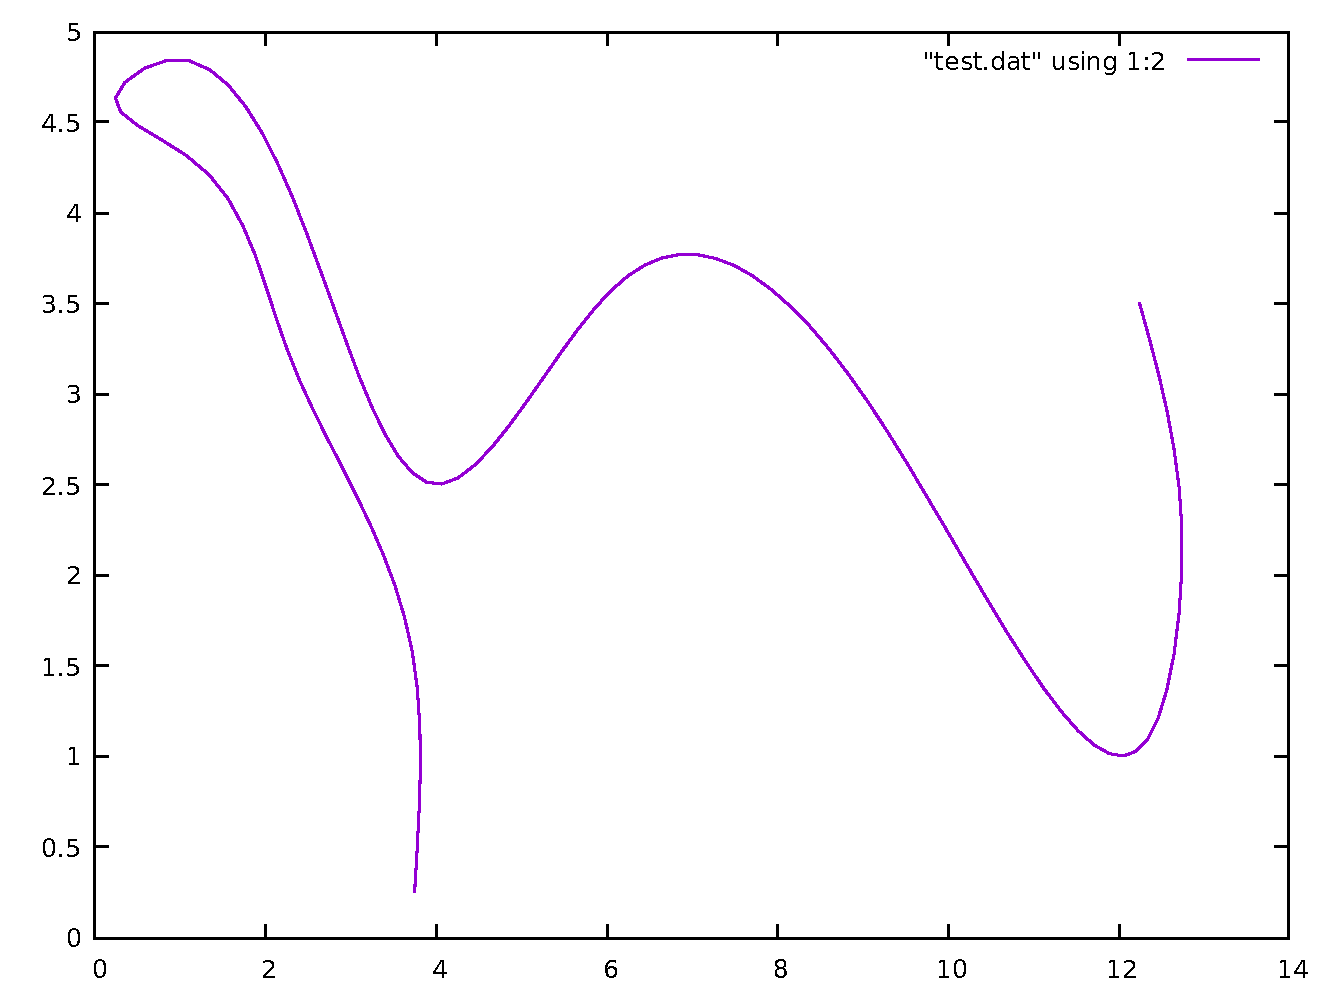
\includegraphics[width=\textwidth]{brontosaurus.pdf}
\end{document}